% FSM controller for the FSMD-style GCD implementation (task2/gcd.vhd)
% Compile standalone with: pdflatex fsm.tex
\documentclass[tikz,border=5mm]{standalone}
\usepackage[T1]{fontenc}
\usetikzlibrary{automata,positioning,arrows.meta,calc}

\begin{document}
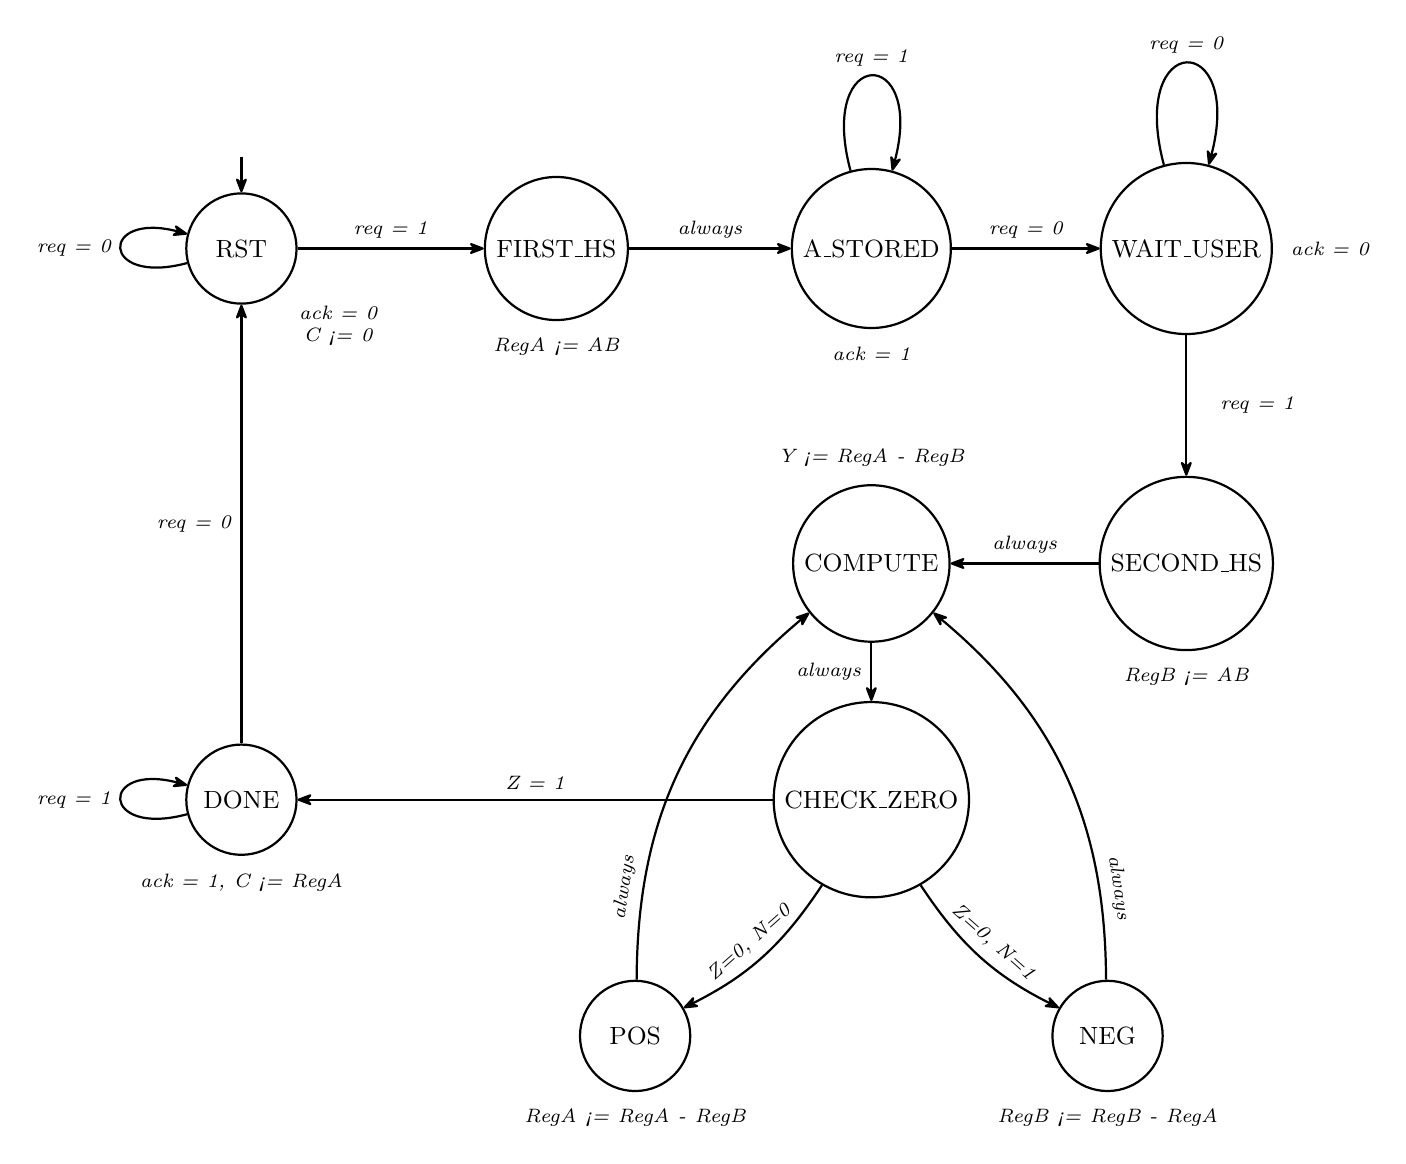
\begin{tikzpicture}[
  >={Stealth[round]},
  every state/.style={draw, thick, minimum size=14mm, font=\small},
  every edge/.style={draw, ->, thick},
  every loop/.style={draw, ->, thick},
  labelnode/.style={font=\scriptsize\itshape, align=center},
]

  % ---------- states ----------
  \node[state, initial, initial where=above, initial text=] (RST)        at (0,4)   {RST};
  \node[state]                          (FIRST_HS)   at (4,4)   {FIRST\_HS};
  \node[state]                          (A_STORED)   at (8,4)   {A\_STORED};
  \node[state]                          (WAIT_USER)  at (12,4)  {WAIT\_USER};
  \node[state]                          (SECOND_HS)  at (12,0)  {SECOND\_HS};
  \node[state]                          (COMPUTE)    at (8,0)   {COMPUTE};
  \node[state]                          (CHECK_ZERO) at (8,-3)  {CHECK\_ZERO};
  \node[state]                          (POS)        at (5,-6)  {POS};
  \node[state]                          (NEG)        at (11,-6) {NEG};
  \node[state]                          (DONE)       at (0,-3)  {DONE};

  % ---------- RT-operation annotations ----------
  % C is 0 in every state except DONE (C <= RegA); only shown in RST and DONE.
  % ack is only shown in the handshake states.
  \node[labelnode, anchor=north west] at ($(RST.south east)+(1mm,-1mm)$) {ack = 0 \\ C <= 0};
  \node[labelnode, below=1mm of FIRST_HS]   {RegA <= AB};
  \node[labelnode, below=1mm of A_STORED]   {ack = 1};
  \node[labelnode, right=1mm of WAIT_USER]  {ack = 0};
  \node[labelnode, below=1mm of SECOND_HS]  {RegB <= AB};
  \node[labelnode, above=1mm of COMPUTE]    {Y <= RegA - RegB};
  \node[labelnode, below=1mm of POS]        {RegA <= RegA - RegB};
  \node[labelnode, below=1mm of NEG]        {RegB <= RegB - RegA};
  \node[labelnode, below=1mm of DONE]       {ack = 1, C <= RegA};

  % ---------- transitions ----------
  \path
    (RST)        edge[loop left]              node[labelnode] {req = 0} (RST)
    (RST)        edge                         node[labelnode, above] {req = 1} (FIRST_HS)
    (FIRST_HS)   edge                         node[labelnode, above] {always} (A_STORED)
    (A_STORED)   edge[loop above]             node[labelnode] {req = 1} (A_STORED)
    (A_STORED)   edge                         node[labelnode, above] {req = 0} (WAIT_USER)
    (WAIT_USER)  edge[loop above]             node[labelnode] {req = 0} (WAIT_USER)
    (WAIT_USER)  edge                         node[labelnode, right=3mm] {req = 1} (SECOND_HS)
    (SECOND_HS)  edge                         node[labelnode, above] {always} (COMPUTE)
    (COMPUTE)    edge                         node[labelnode, left] {always} (CHECK_ZERO)
    (CHECK_ZERO) edge[bend left=15]           node[labelnode, above, sloped] {Z=0, N=0} (POS)
    (CHECK_ZERO) edge[bend right=15]          node[labelnode, above, sloped] {Z=0, N=1} (NEG)
    (CHECK_ZERO) edge                         node[labelnode, above] {Z = 1} (DONE)
    (POS)        edge[bend left=25]           node[labelnode, sloped, above, pos=0.2] {always} (COMPUTE)
    (NEG)        edge[bend right=25]          node[labelnode, sloped, above, pos=0.2] {always} (COMPUTE)
    (DONE)       edge[loop left]              node[labelnode] {req = 1} (DONE)
    (DONE)       edge                         node[labelnode, left] {req = 0} (RST)
  ;

  % ---------- global asynchronous reset note ----------
  %\node[labelnode, align=left, text width=6.5cm] at (16.5,-2) {
  %  Asynchronous \texttt{reset = 1} forces the FSM\\
  %  to state RST from every state (not drawn\\
  %  on every arrow to keep the diagram readable).
  %};

\end{tikzpicture}
\end{document}
